\subsection*{Задание}

Дата отчета 8 мая.


Отметить как выполненные все работы, которые должны были завершиться на эту дату, кроме:

\begin{enumerate}
    \item С 11 марта доступность системного аналитика уменьшилась до 70\%, так как его привлекли к подготовке другого проекта.
    \item Чтобы компенсировать отставание программистских задач по созданию ядра GIS и базы объектов, возникших из-за снижения доступности системного аналитика, с 18 марта был дополнительно нанят программист-стажер, стандартная ставка которого составляет 3 р/час, ставка сверхурочных – 5 р/час, а затраты на использование – 20 руб.
    \item Задача №4 фактически завершилась 28 марта.
    \item Фактическая длительность задачи №5 оказалась на 20\% больше.
    \item Задача №17 выполнена на 30\%.
    \item С 1 апреля на 10\% выросла зарплата мультимедиа корреспондента.
    \item С 1 апреля на 10\% увеличилась стоимость аренды сервера.
    \item Для задачи мультимедиа наполнения купили лицензию на специализированное ПО стоимостью 5000 рублей в год и потратили 300 рублей на его инсталляцию и настройку.
\end{enumerate}

\subsection*{Информация о проекте до внесения изменений}

До внесения изменений стоимость проекта составляла 48 456 рублей, дата окончания проекта --- 24.07.2024, общая длительность проекта --- 19,24 недели. Проект укладывался в рамки как по срокам завершения, так и по затратам.

\begin{figure}[h!]
	\begin{center}
		
\includegraphics[scale=0.6]{inc/img/p_1.png}
	\end{center}
	\captionsetup{justification=centering}
	\label{fig:u3}
\end{figure}

\subsection*{Отчет на дату 8 мая}

Задан новый отчет на дату 8 мая.

\begin{figure}[h!]
	\begin{center}
		
\includegraphics[scale=0.8]{inc/img/p_2.png}
	\end{center}
	\captionsetup{justification=centering}
	\label{fig:u3}
\end{figure}

\textbf{1. С 11 марта доступность системного аналитика уменьшилась до 70\%, так как его привлекли к подготовке другого проекта.}

Была изменена доступность ресурса <<Системный аналитик>> в соответствии с заданием.

\begin{figure}[h!]
	\begin{center}
		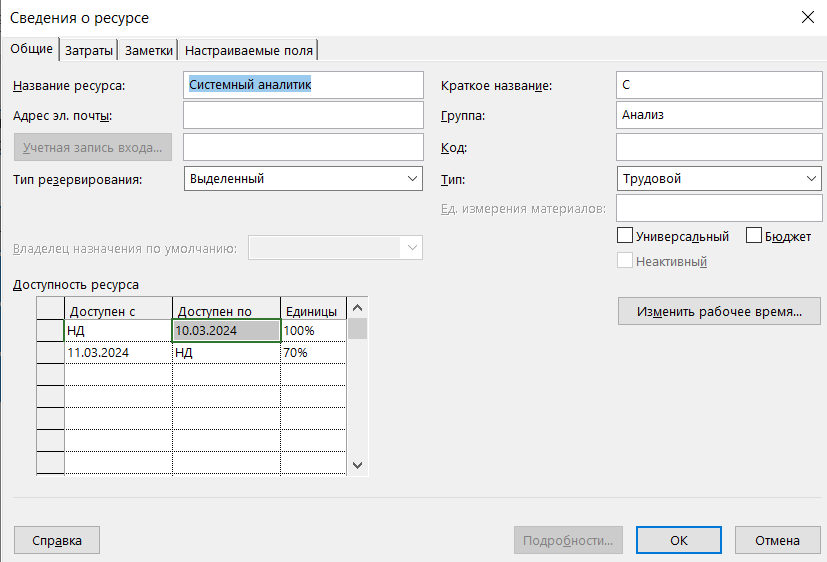
\includegraphics[scale=0.8]{inc/img/p_3.png}
	\end{center}
	\captionsetup{justification=centering}
	\label{fig:u3}
\end{figure}

\newpage

В связи с изменением доступности возникла перегрузка ресурса <<Системный аналитик>> в задачах <<Анализ и построение структуры базы объектов>> и <<Анализ и проектирование ядра>>.

\begin{figure}[h!]
	\begin{center}
		
\includegraphics[scale=0.7]{inc/img/p_4.jpg}
	\end{center}
	\captionsetup{justification=centering}
	\label{fig:u3}
\end{figure}

После устранения перегрузки с помощью автоматического выравнивания (по дням) появилась перегрузка у web-дизайнера в задаче <<Разработка дизайна сайта>>. Перегрузка была устранена удалением web-дизайнера с совещания 17 (так как совещания проходят в конкретное время и сдвинуть их невозможно).

\begin{figure}[h!]
	\begin{center}
		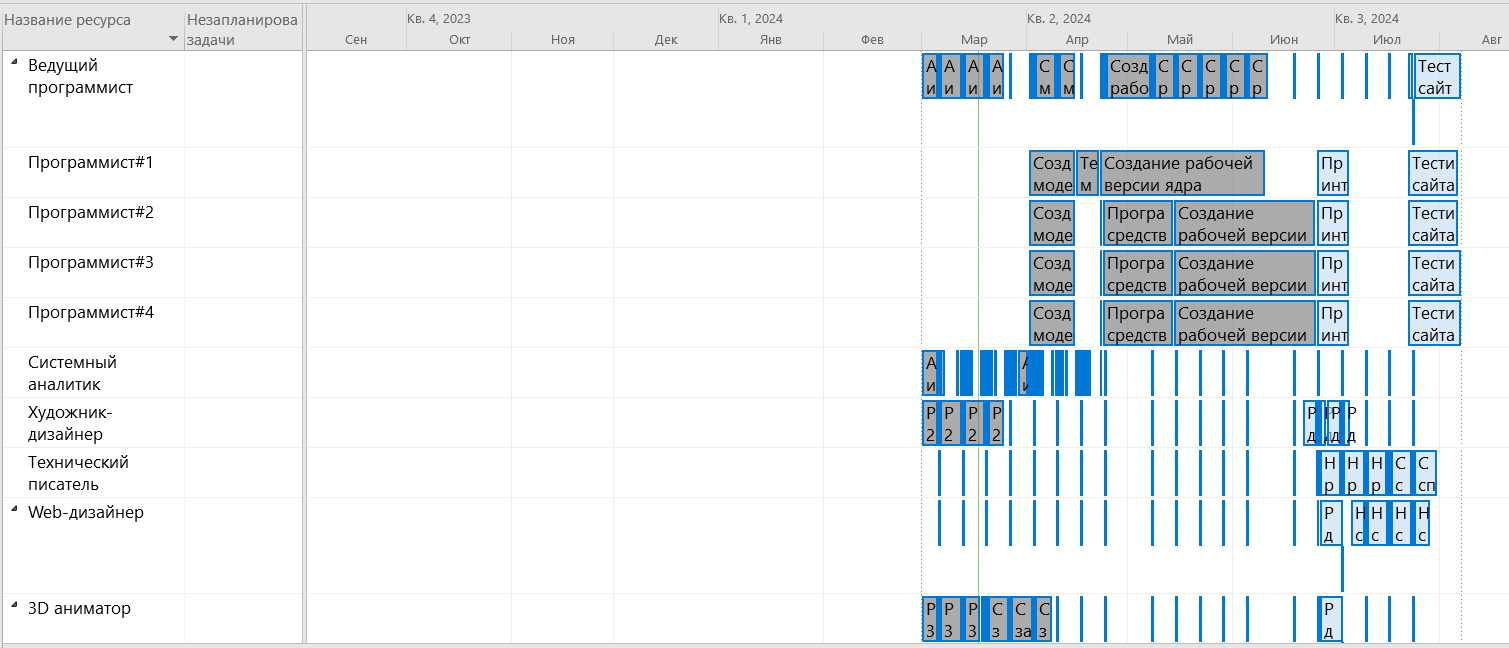
\includegraphics[scale=0.4]{inc/img/p_5.png}
	\end{center}
	\captionsetup{justification=centering}
	\label{fig:u3}
\end{figure}

В результате незначительно увеличилась стоимость проекта (до 48 538 рублей), а также изменилась дата окончания проекта --- теперь это 2 августа 2024 года.

\begin{figure}[h!]
	\begin{center}
		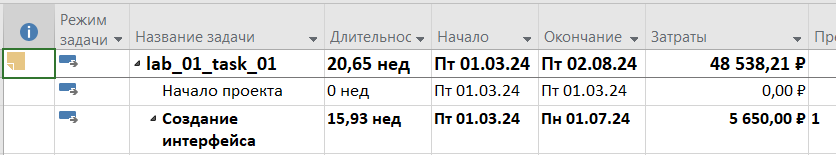
\includegraphics[scale=0.6]{inc/img/p_6.png}
	\end{center}
	\captionsetup{justification=centering}
	\label{fig:u3}
\end{figure}

\newpage

\textbf{2. Чтобы компенсировать отставание программистских задач по созданию ядра GIS и базы объектов, возникших из-за снижения доступности системного аналитика, с 18 марта был дополнительно нанят программист-стажер, стандартная ставка которого составляет 3 р/час, ставка сверхурочных – 5 р/час, а затраты на использование – 20 руб.}

Был создан новый ресурс <<Программист-стажер>> в соответствии с заданием.

\begin{figure}[h!]
	\begin{center}
		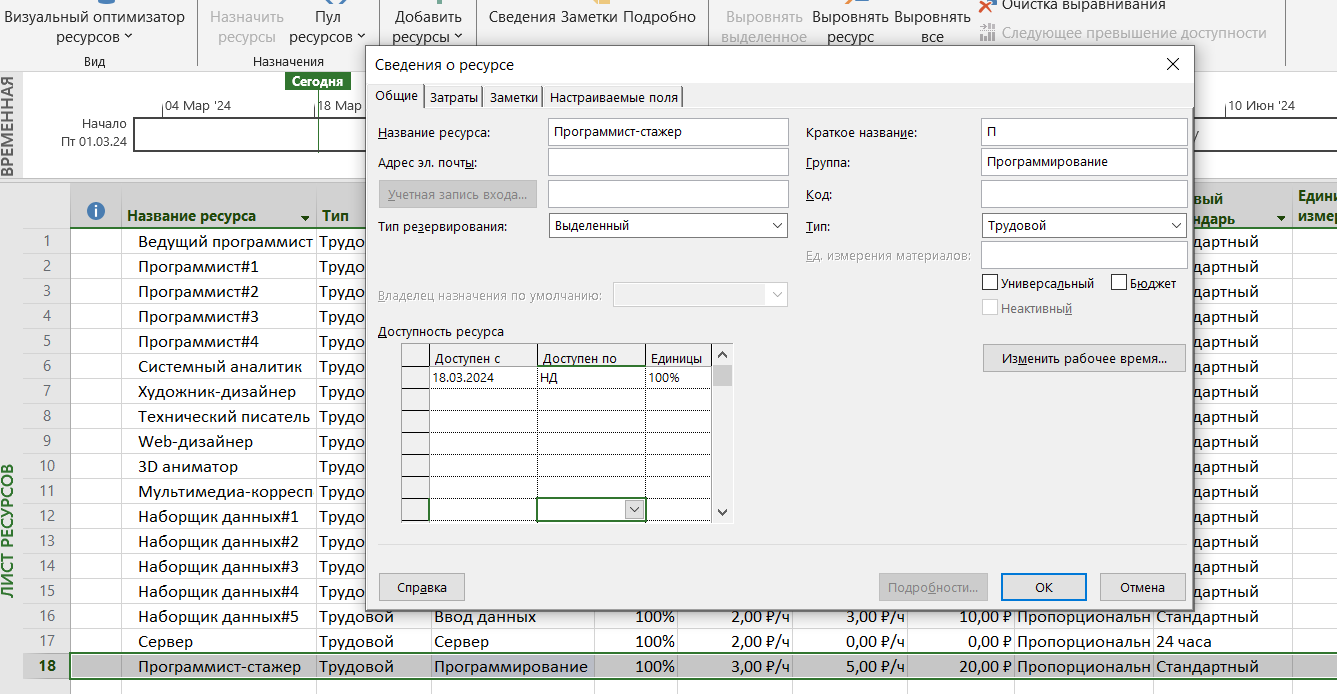
\includegraphics[scale=0.45]{inc/img/p_7.png}
	\end{center}
	\captionsetup{justification=centering}
	\label{fig:u3}
\end{figure}

Ресурс был добавлен в задачи <<Программирование средств обработки базы объектов>>, <<Создание модели ядра>>, <<Тестирование модели ядра>>, <<Создание рабочей версии ядра>>, <<Программирование интерфейса>>, <<Тестирование сайта>>.

\begin{figure}[h!]
	\begin{center}
		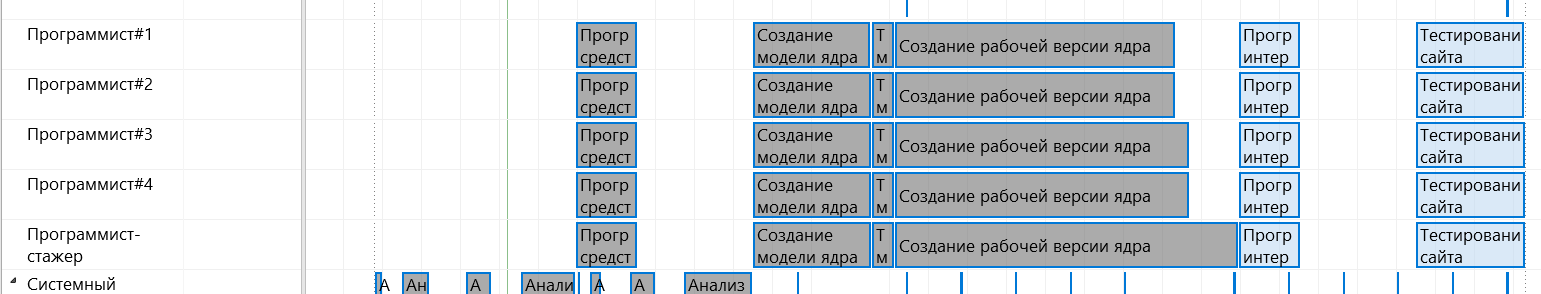
\includegraphics[scale=0.35]{inc/img/p_8.png}
	\end{center}
	\captionsetup{justification=centering}
	\label{fig:u3}
\end{figure}

При добавлении ресурса использовался параметр <<Сохранить длительность и сохранить объем трудозатрат>>, так как стажер нанят в помощь остальным разработчикам.

\begin{figure}[h!]
	\begin{center}
		
\includegraphics[scale=0.5]{inc/img/p_10.png}
	\end{center}
	\captionsetup{justification=centering}
	\label{fig:u3}
\end{figure}

В результате стоимость проекта уменьшилась до 46 850 рублей, новый строк окончания проекта --- 26.07.2024. 

\begin{figure}[h!]
	\begin{center}
		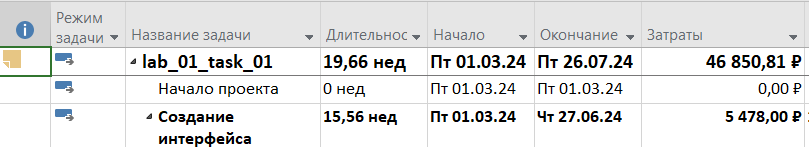
\includegraphics[scale=0.5]{inc/img/p_9.png}
	\end{center}
	\captionsetup{justification=centering}
	\label{fig:u3}
\end{figure}

\textbf{3. Задача №4 фактически завершилась 28 марта.}

Срок завершения задачи <<Разработка 2D графических элементов>> был по плану был 25 марта 2024 года.

\begin{figure}[h!]
	\begin{center}
		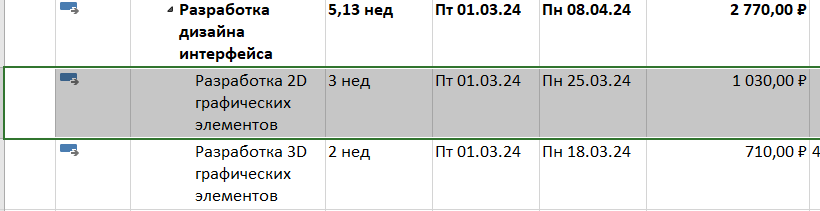
\includegraphics[scale=0.5]{inc/img/p_11.png}
	\end{center}
	\captionsetup{justification=centering}
	\label{fig:u3}
\end{figure}

Задача была обновлена, установлен фактический срок завершения --- 28.03.2024.

\begin{figure}[h!]
	\begin{center}
		
\includegraphics[scale=0.65]{inc/img/p_12.png}
	\end{center}
	\captionsetup{justification=centering}
	\label{fig:u3}
\end{figure}

В результате изменилась длительность выполнения задачи, но дата завершения проекта и его финальная стоимость не поменялись.

\begin{figure}[h!]
	\begin{center}
		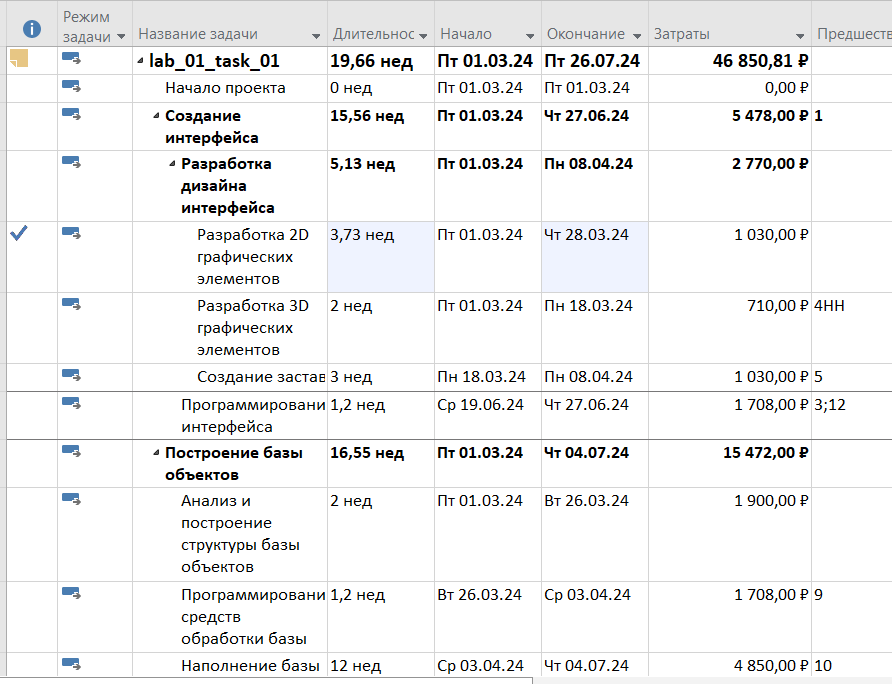
\includegraphics[scale=0.6]{inc/img/p_13.png}
	\end{center}
	\captionsetup{justification=centering}
	\label{fig:u3}
\end{figure}

\newpage

\textbf{4. Фактическая длительность задачи №5 оказалась на 20\% больше.}

Первоначально длительность задачи <<Разработка 3D графических элементов>> составляла 2 недели, планируемые сроки выполнения --- с 1 марта по 18 марта 2024 года.

\begin{figure}[h!]
	\begin{center}
		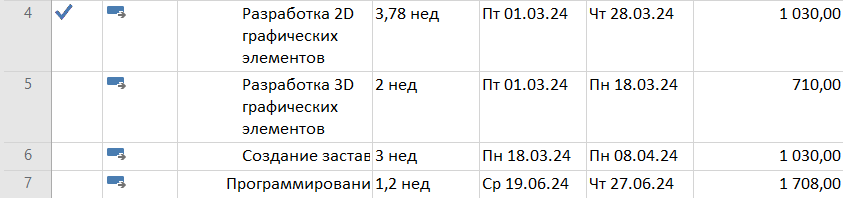
\includegraphics[scale=0.6]{inc/img/p_14.png}
	\end{center}
	\captionsetup{justification=centering}
	\label{fig:u3}
\end{figure}

Длительность задачи была обновлена. Фактическая длительность составила 2.4 недели, новые строки выполнения --- с 1 марта по 20 марта 2024 года. При этом стоимость выполнения задачи не изменилась.

\begin{figure}[h!]
	\begin{center}
		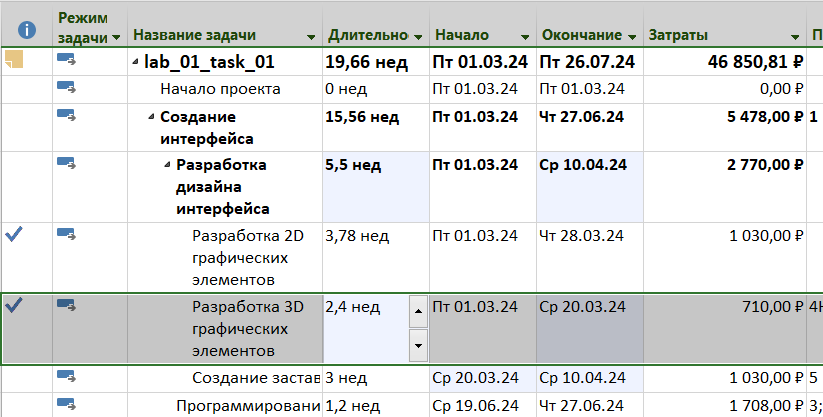
\includegraphics[scale=0.6]{inc/img/p_15.png}
	\end{center}
	\captionsetup{justification=centering}
	\label{fig:u3}
\end{figure}

В результате сроки выполнения проекта изменены не были, стоимость проекта осталась прежней.

\newpage


\textbf{5. Задача №17 выполнена на 30\%.}

Задача <<Создание мультимедия наполнения>> была обновлена, выставлен процент выполнения --- 30\%.

\begin{figure}[h!]
	\begin{center}
		
\includegraphics[scale=0.6]{inc/img/p_16.png}
	\end{center}
	\captionsetup{justification=centering}
	\label{fig:u3}
\end{figure}

\textbf{6. С 1 апреля на 10\% выросла зарплата мультимедиа корреспондента.}

Зарплата мультимедиа-корреспондента была изменена согласно заданию. Новая ставка --- 3.3 руб/час.

\begin{figure}[h!]
	\begin{center}
		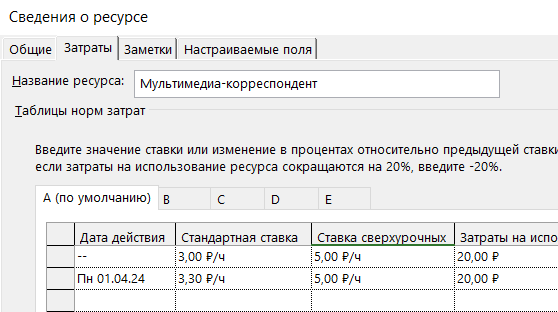
\includegraphics[scale=0.7]{inc/img/p_18.png}
	\end{center}
	\captionsetup{justification=centering}
	\label{fig:u3}
\end{figure}

В результате стоимость проекта увеличилась до 46 992 рублей, сроки проекта не изменились.

\begin{figure}[h!]
	\begin{center}
		
\includegraphics[scale=0.7]{inc/img/p_19.png}
	\end{center}
	\captionsetup{justification=centering}
	\label{fig:u3}
\end{figure}

\textbf{7. С 1 апреля на 10\% увеличилась стоимость аренды сервера.}

Стоимость аренды сервера была изменена согласно заданию.

\begin{figure}[h!]
	\begin{center}
		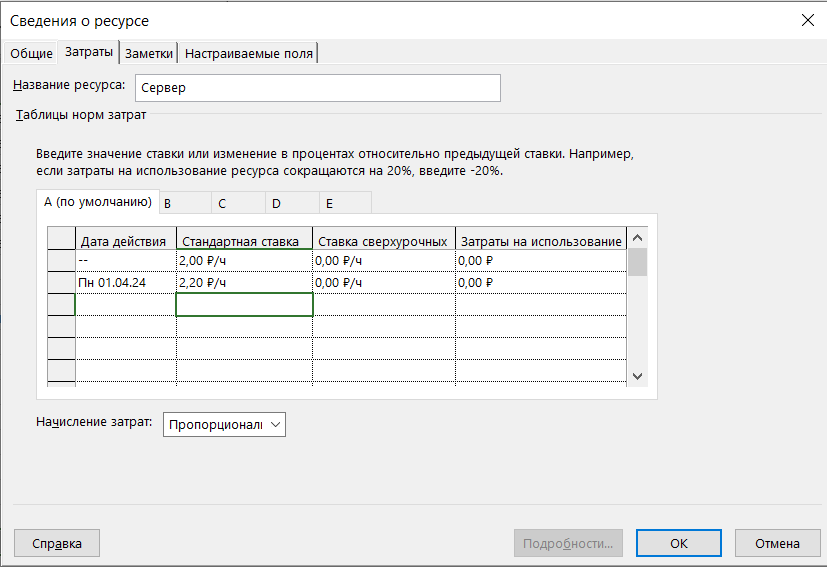
\includegraphics[scale=0.65]{inc/img/p_20.png}
	\end{center}
	\captionsetup{justification=centering}
	\label{fig:u3}
\end{figure}

В результате выросла стоимость выполнения проекта, общая сумма составила 47~375 рублей.

\begin{figure}[h!]
	\begin{center}
		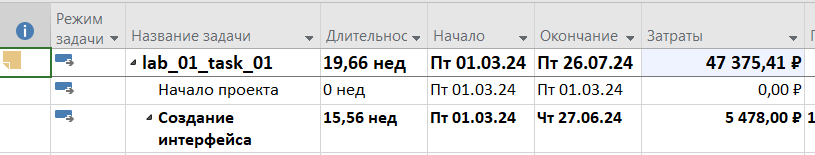
\includegraphics[scale=0.7]{inc/img/p_21.png}
	\end{center}
	\captionsetup{justification=centering}
	\label{fig:u3}
\end{figure}

\newpage

\textbf{8. Для задачи мультимедиа наполнения купили лицензию на специализированное ПО стоимостью 5000 рублей в год и потратили 300 рублей на его инсталляцию и настройку.}

Был создан новый ресурс <<Специализированное ПО>> согласно заданию.

\begin{figure}[h!]
	\begin{center}
		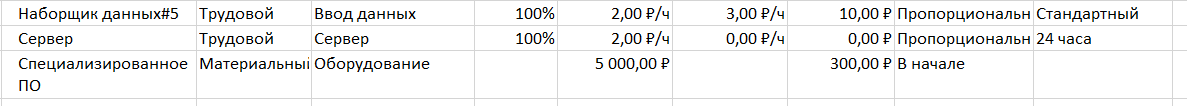
\includegraphics[scale=0.5]{inc/img/p_22.png}
	\end{center}
	\captionsetup{justification=centering}
	\label{fig:u3}
\end{figure}

Ресурс был добавлен в задачу <<Создание мультимедиа-наполнения>>, в результате стоимость задачи выросла до 6~112 рублей.

\begin{figure}[h!]
	\begin{center}
		
\includegraphics[scale=0.6]{inc/img/p_23.png}
	\end{center}
	\captionsetup{justification=centering}
	\label{fig:u3}
\end{figure}

Общая стоимость проекта увеличилась до 52~675 рублей, что превыщает бюджет проекта на 2~675 рублей и требует оптимизации.

\begin{figure}[h!]
	\begin{center}
		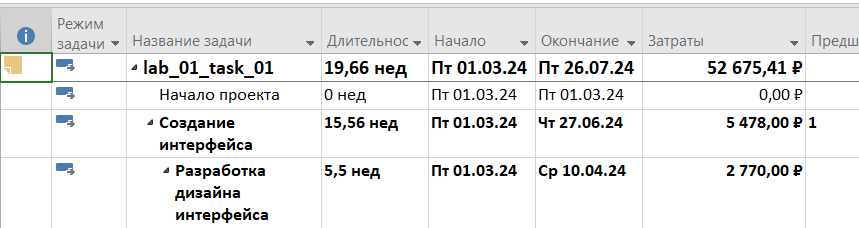
\includegraphics[scale=0.6]{inc/img/p_24.png}
	\end{center}
	\captionsetup{justification=centering}
	\label{fig:u3}
\end{figure}

\textbf{9. Все остальные работы, которые должны были завершиться на 8 мая,
отмечены как выполненные.}

\begin{figure}[h!]
	\begin{center}
		
\includegraphics[scale=0.6]{inc/img/p_25.png}
	\end{center}
	\captionsetup{justification=centering}
	\label{fig:u3}
\end{figure}

\begin{figure}[h!]
	\begin{center}
		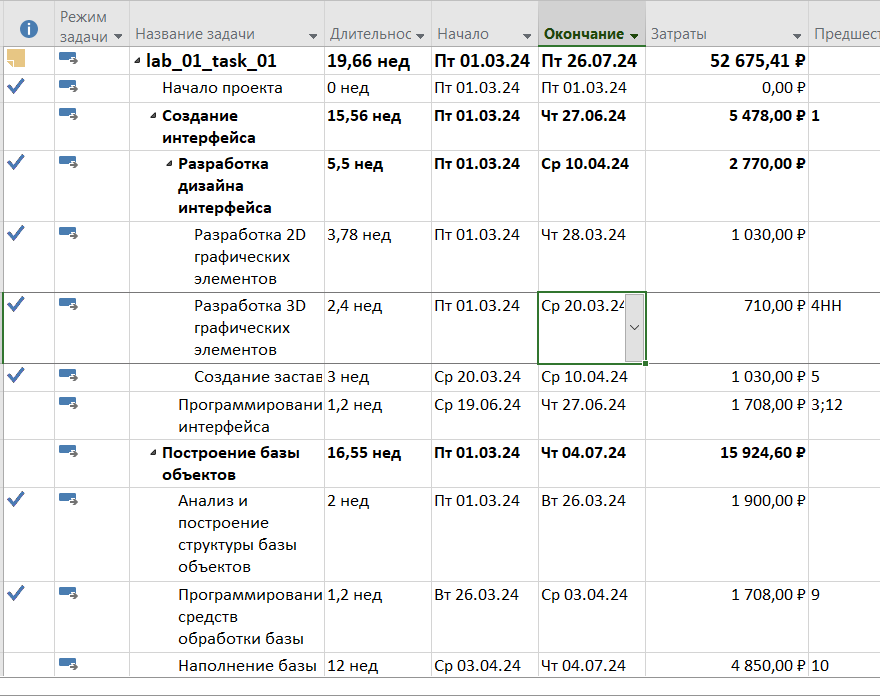
\includegraphics[scale=0.6]{inc/img/p_26.png}
	\end{center}
	\captionsetup{justification=centering}
	\label{fig:u3}
\end{figure}

\subsection*{Сравнение плановых и фактических показателей}

Стоимость проекта существенно увеличилась, дата
начала – не изменилась, срок окончания сдвинулся на 2 дня вперед. Длительность проекта (19.66 недель) укладывается в установленные строки, затраты на проект (52~675 руб) не укладываются в установленные рамки (50000 и 6 месяцев, соответственно).

\begin{figure}[h!]
	\begin{center}
		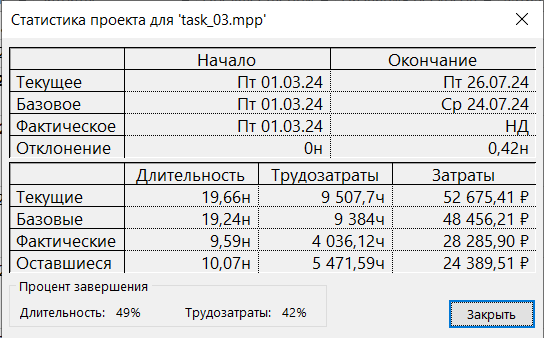
\includegraphics[scale=0.7]{inc/img/p_27.png}
	\end{center}
	\captionsetup{justification=centering}
	\label{fig:u3}
\end{figure}

\subsection*{Линия прогресса}

На основе базового плана:

\begin{figure}[h!]
	\begin{center}
		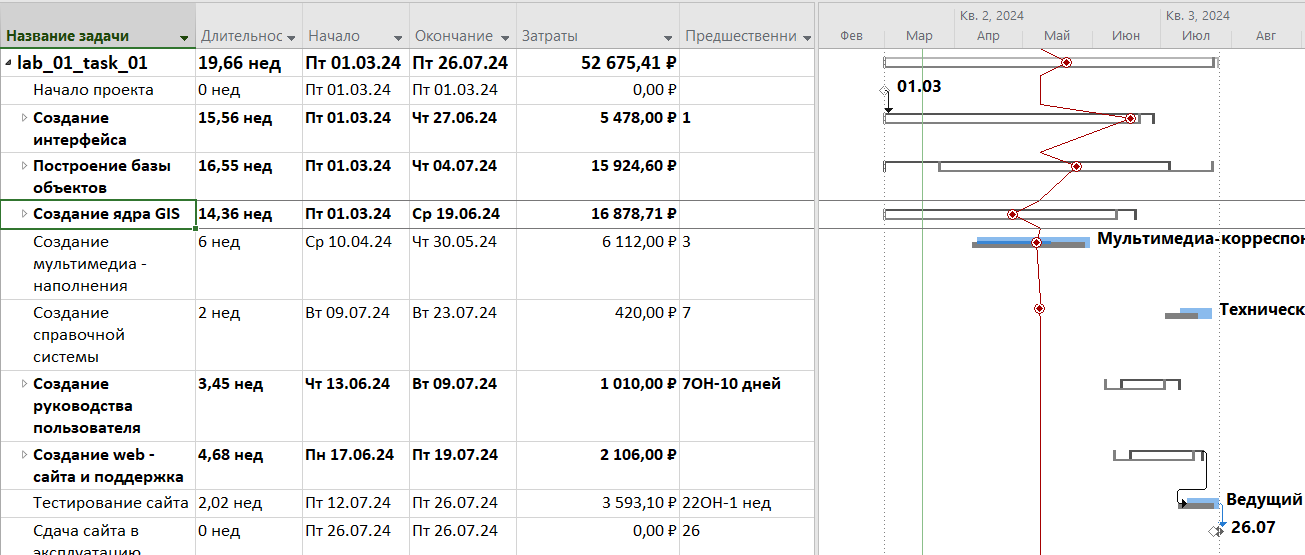
\includegraphics[scale=0.45]{inc/img/p_28.png}
	\end{center}
	\captionsetup{justification=centering}
	\label{fig:u3}
\end{figure}

Имеются изгибы как вправо, так и влево, то есть некоторые задачи выполняются с опережением (например, создание интерфейса, построение базы объектов), а некоторые – с запаздыванием (создание ядра GIS). 

Задача <<Наполнение базы объектов>> начнется раньше благодаря найму в команду стажера-программиста, который помог группе программирование закончить все работы по программированию средств обработки базы раньше планируемого срока. Поэтому задача <<Построение базы объектов>> выполняется с опережением.

Задача <<Создание ядра GIS>> задерживается из-за снижения доступности аналитика до 70\% (в результате все задачи по созданию ядра были смещены, последняя задача --- создание рабочей версиии ядра теперь начнется не 15 апреля, а 6 мая).

Остальные задачи выполняются согласно базовому плану.

\subsection*{Стратегия устранения временных отклонений}

Отклонения от заданного плана наблюдаются в одной единственной задаче --- <<Создание рабочей версии ядра>>. Так как задача будет завершена всего на 2 дня позже, а также исходя из того, что проект укладывается в установленные строки в 6 месяцев, было принято решение, что оптимизировать это отклонение не имеет смысла.

\subsection*{Стратегия устранения отклонений от бюджета}

На момент отчета 8 мая есть превыщение бюджета проекта на 2 675 рублей. Для устранения этого превышения были проведены следующие действия:

\begin{enumerate}
    \item Был нанят еще один программист-стажер, который помогает группе программистов в решении задач по создании ядра GIS. Это позволило выполнять эти задачи быстрее, а значит сократить расходы на выполнение.
    \item Был нанят еще один наборшик данных, в результате удалось снизить затраты на выполнение задачи <<Наполнение базы объектов>>.
\end{enumerate}

В итоге были получены следующие характеристики проекта:

\begin{figure}[h!]
	\begin{center}
		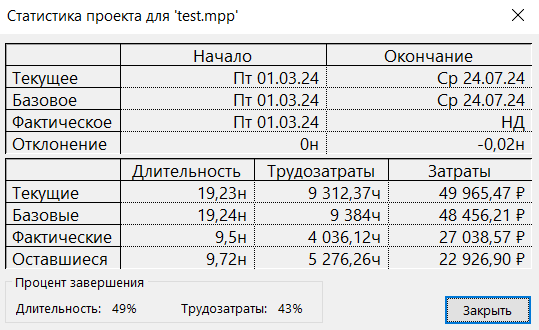
\includegraphics[scale=0.7]{inc/img/p_29.png}
	\end{center}
	\captionsetup{justification=centering}
	\label{fig:u3}
\end{figure}

Стоимость проекта увеличилась до 49 965 рублей, длительность проекта не изменилась. Проект укладывается в установленные рамки.
